\chapter{Estereoquímica: quiralidade e isômeros}\label{ch:g12:stereochemistry}

As folhas de hortelã e as sementes de alcaravia não têm nada a ver no
cheiro: uma tem o cheiro fresco de chiclete, a outra o cheiro quente do
pão de centeio. No entanto, a \omterm{def:g7:atoms-and-molecules:molecule}{molécula} responsável por cada cheiro é a
mesma carvona, feita dos mesmos \omterm{def:g7:atoms-and-molecules:atom}{átomos} ligados na mesma ordem. As duas
carvonas só diferem como uma mão esquerda difere de uma mão direita:
cada uma é a imagem no espelho da outra. O nosso nariz, feito de
\omterm{def:g7:atoms-and-molecules:molecule}{moléculas} que também têm ``mão'', distingue uma da outra. Este capítulo
aprende a ver as \omterm{def:g7:atoms-and-molecules:molecule}{moléculas} em três dimensões.

\begin{recall}
A geometria das \omterm{def:g7:atoms-and-molecules:molecule}{moléculas}, e as cunhas cheias e tracejadas que as
desenham no espaço (\cref{ch:g10:lewis-and-shape}). Os \omterm{def:g11:organic-skeletons:isomer}{isômeros
constitucionais} (\cref{ch:g11:organic-skeletons}). Os \omterm{def:g11:functional-groups:functional-group}{grupos funcionais}
(\cref{ch:g11:functional-groups}).
\end{recall}

\begin{omfigure}
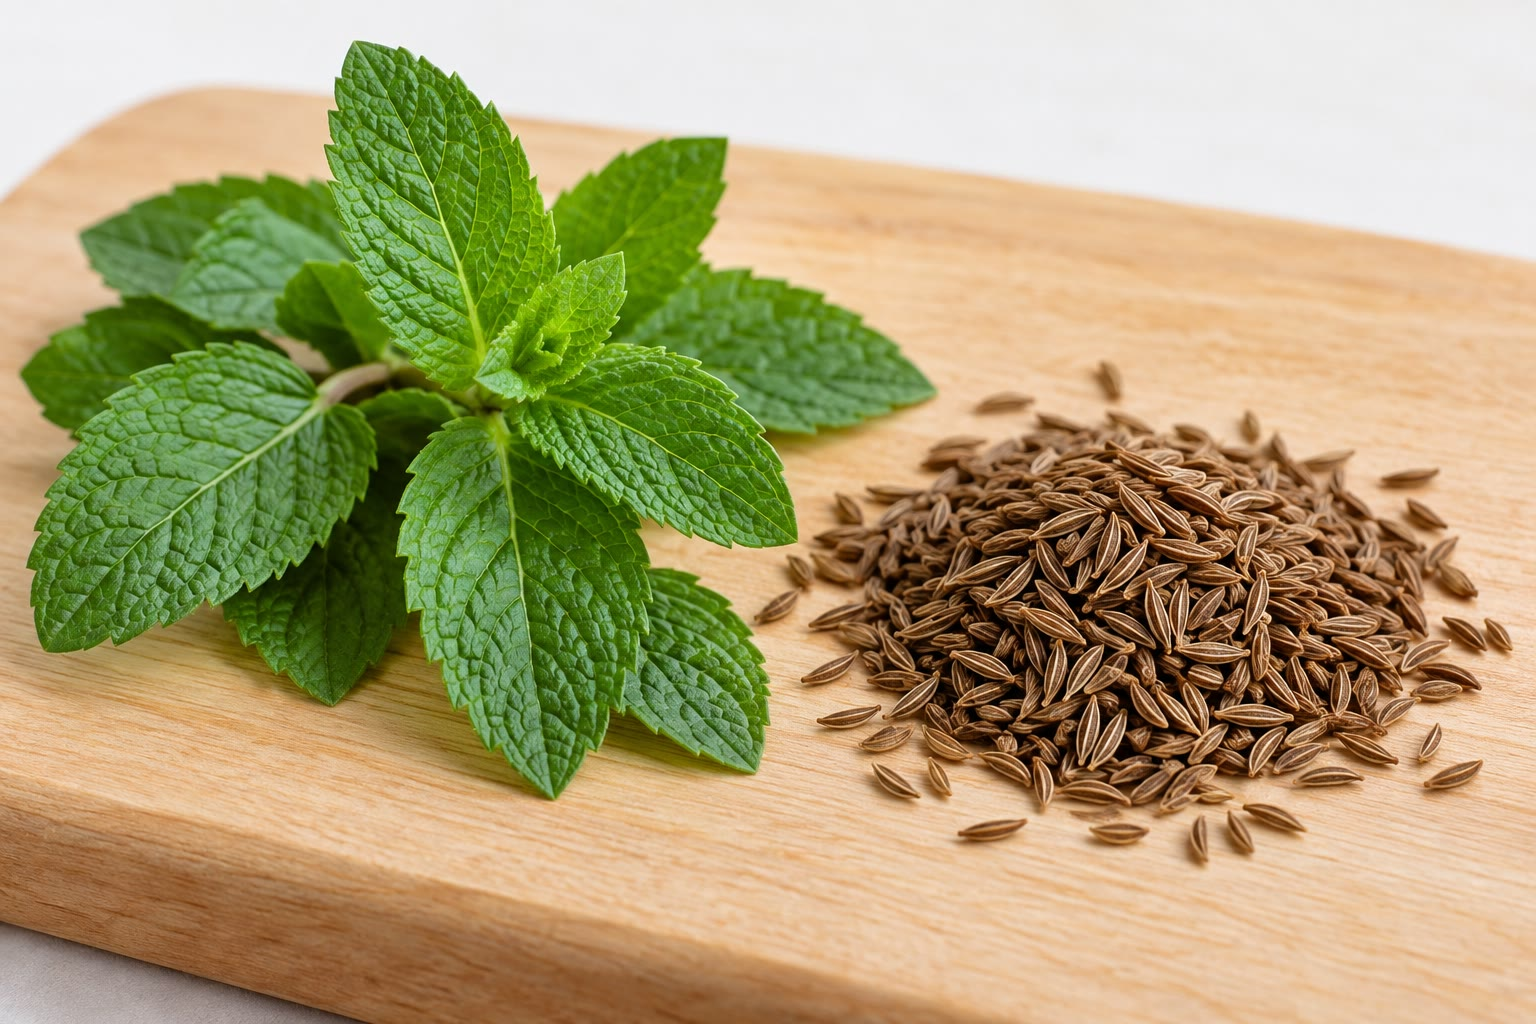
\includegraphics[width=0.48\linewidth]{images/book1/ai/g12-mint-caraway.jpg}

{\small Hortelã e alcaravia: duas \omterm{def:g7:atoms-and-molecules:molecule}{moléculas} imagens no espelho uma da
outra, dois cheiros.}
\end{omfigure}

\section{As moléculas no espaço}

\begin{definition}[Estereoisômeros]\label{def:g12:stereochemistry:stereoisomer}
\emph{Estereoisômeros}\index{estereoisomeros@estereoisômeros} são \omterm{def:g7:atoms-and-molecules:molecule}{moléculas} com a mesma
fórmula e a mesma sequência de \omterm{def:g7:atoms-and-molecules:atom}{átomos} ligados, que só diferem pela
disposição dos seus \omterm{def:g7:atoms-and-molecules:atom}{átomos} no espaço.
\end{definition}

\begin{definition}[Representação de Cram]\label{def:g12:stereochemistry:cram}
Na \emph{representação de Cram}\index{representacao de Cram@representação de Cram} de um \omterm{def:g7:atoms-and-molecules:atom}{átomo}
de carbono com quatro ligações simples, duas ligações são desenhadas no
plano do papel como traços simples, formando um ângulo, a ligação que
aponta para o leitor como uma cunha cheia e a ligação que se afasta dele
como uma cunha tracejada.
\end{definition}

\section{A quiralidade}

\begin{definition}[Quiral, carbono assimétrico]\label{def:g12:stereochemistry:chiral}
Um objeto ou uma \omterm{def:g7:atoms-and-molecules:molecule}{molécula} é \emph{quiral}\index{quiral} se não pode ser
sobreposto à sua imagem no espelho, como uma mão. Um \omterm{def:g7:atoms-and-molecules:atom}{átomo} de carbono
ligado a quatro \omterm{def:g7:atoms-and-molecules:atom}{átomos} ou grupos diferentes é um \emph{carbono
assimétrico}\index{carbono assimetrico@carbono assimétrico}; ele costuma ser marcado com um
asterisco.
\end{definition}

\begin{proposition}[Um carbono assimétrico torna uma molécula quiral]\label{prop:g12:stereochemistry:one-carbon}
Uma \omterm{def:g7:atoms-and-molecules:molecule}{molécula} com exatamente um \omterm{def:g12:stereochemistry:chiral}{carbono assimétrico} é \omterm{def:g12:stereochemistry:chiral}{quiral}.
\end{proposition}

\begin{proof}
Admitido: trocar dois dos quatro grupos diferentes em volta do \omterm{def:g12:stereochemistry:chiral}{carbono
assimétrico} dá a imagem no espelho, e nenhuma rotação da \omterm{def:g7:atoms-and-molecules:molecule}{molécula}
inteira consegue trazê-la de volta, já que os quatro grupos são todos
diferentes.
\end{proof}

\begin{definition}[Enantiômeros, mistura racêmica]\label{def:g12:stereochemistry:enantiomer}
Dois \omterm{def:g12:stereochemistry:stereoisomer}{estereoisômeros} que são imagens no espelho um do outro e não são
sobreponíveis são \emph{enantiômeros}\index{enantiomeros@enantiômeros}. Uma \omterm{def:g6:pure-substances-and-mixtures:mixture}{mistura} de
quantidades iguais de dois enantiômeros é uma \emph{mistura
racêmica}\index{mistura racemica@mistura racêmica}.
\end{definition}

\begin{omfigure}
\setchemfig{atom sep=2.2em}
\begin{tikzpicture}[font=\small]
  \node at (-2.4,0) {\chemfig{C(-[2]COOH)(-[4]H_3C)(<[:-30]OH)(<:[:-150]H)}};
  \node at (2.4,0) {\chemfig{C(-[2]COOH)(-[0]CH_3)(<[:-150]HO)(<:[:-30]H)}};
  \draw[dashed, omDef, thick] (0,-1.5) -- (0,1.6) node[above] {espelho};
  \node[anchor=north] at (-2.4,-1.4) {ácido lático, A};
  \node[anchor=north] at (2.4,-1.4) {sua imagem no espelho, B};
\end{tikzpicture}

{\small Os dois \omterm{def:g12:stereochemistry:enantiomer}{enantiômeros} do ácido lático, \ce{CH3-CH(OH)-COOH}, na
\omterm{def:g12:stereochemistry:cram}{representação de Cram}. O carbono central é assimétrico (\ce{H}, \ce{OH},
\ce{CH3}, \ce{COOH}). Nenhuma rotação transforma A em B: eles são tão
diferentes quanto uma mão esquerda e uma mão direita.}
\end{omfigure}

\begin{method}[Uma molécula é quiral?]\label{met:g12:stereochemistry:chiral}
\begin{enumerate}
  \item Procure os \omterm{def:g12:stereochemistry:chiral}{carbonos assimétricos}: um carbono com quatro grupos
        diferentes. Nenhum: a \omterm{def:g7:atoms-and-molecules:molecule}{molécula} (neste livro) não é \omterm{def:g12:stereochemistry:chiral}{quiral}.
  \item Exatamente um: a \omterm{def:g7:atoms-and-molecules:molecule}{molécula} é \omterm{def:g12:stereochemistry:chiral}{quiral}.
  \item Dois ou mais: procure um plano que corte a \omterm{def:g7:atoms-and-molecules:molecule}{molécula} em duas
        metades espelhadas, numa das suas formas; se houver um, a
        \omterm{def:g7:atoms-and-molecules:molecule}{molécula} não é \omterm{def:g12:stereochemistry:chiral}{quiral}; senão, ela é.
\end{enumerate}
\end{method}

\begin{remark}[Mesmas propriedades, cheiros diferentes]\label{rem:g12:stereochemistry:same}
% ledger: smell:carvone-R, smell:carvone-S
Dois \omterm{def:g12:stereochemistry:enantiomer}{enantiômeros} têm as mesmas temperaturas de fusão e de ebulição, a
mesma \omterm{def:g6:solutions-and-solubility:solubility}{solubilidade}, os mesmos espectros: toda medida feita com algo que
não é \omterm{def:g12:stereochemistry:chiral}{quiral} dá o mesmo resultado para os dois. Eles só diferem quando
encontram algo \omterm{def:g12:stereochemistry:chiral}{quiral}, como a luz polarizada, que eles desviam em
sentidos opostos, ou os receptores do nariz: uma carvona tem cheiro de
hortelã, o seu \omterm{def:g12:stereochemistry:enantiomer}{enantiômero}, de alcaravia.
\end{remark}

\section{Os diastereoisômeros}

\begin{definition}[Diastereoisômeros]\label{def:g12:stereochemistry:diastereomer}
\omterm{def:g12:stereochemistry:stereoisomer}{Estereoisômeros} que não são imagens no espelho um do outro são
\emph{diastereoisômeros}\index{diastereoisomeros@diastereoisômeros}. Ao contrário dos
\omterm{def:g12:stereochemistry:enantiomer}{enantiômeros}, os diastereoisômeros têm propriedades físicas diferentes.
\end{definition}

\begin{proposition}[Contar os estereoisômeros]\label{prop:g12:stereochemistry:count}
Uma \omterm{def:g7:atoms-and-molecules:molecule}{molécula} com $n$ \omterm{def:g12:stereochemistry:chiral}{carbonos assimétricos} tem no máximo $2^n$
\omterm{def:g12:stereochemistry:stereoisomer}{estereoisômeros}. Há menos quando a \omterm{def:g7:atoms-and-molecules:molecule}{molécula} tem duas metades iguais:
então uma das combinações tem um plano de simetria e não é \omterm{def:g12:stereochemistry:chiral}{quiral} (uma
forma \emph{meso}).
\end{proposition}

\begin{proof}
Cada \omterm{def:g12:stereochemistry:chiral}{carbono assimétrico} pode ter duas disposições, independentemente
dos outros: $2 \times 2 \times \dots \times 2 = 2^n$ combinações. Quando
duas combinações são a mesma \omterm{def:g7:atoms-and-molecules:molecule}{molécula}, a contagem diminui.
\end{proof}

\begin{omfigure}
\setchemfig{atom sep=1.9em}
\begin{tabular}{ccc}
\chemfig{HOOC-[:-30]C(<[:-90]OH)-[:30]C(<[:90]OH)-[:-30]COOH} &
\chemfig{HOOC-[:-30]C(<:[:-90]OH)-[:30]C(<:[:90]OH)-[:-30]COOH} &
\chemfig{HOOC-[:-30]C(<[:-90]OH)-[:30]C(<:[:90]OH)-[:-30]COOH} \\[4pt]
\small ácido L-tartárico & \small ácido D-tartárico & \small ácido meso-tartárico \\
\small (\omterm{def:g12:stereochemistry:chiral}{quiral}) & \small (\omterm{def:g12:stereochemistry:chiral}{quiral}, imagem no espelho do L) & \small (não \omterm{def:g12:stereochemistry:chiral}{quiral})
\end{tabular}

{\small Os três \omterm{def:g12:stereochemistry:stereoisomer}{estereoisômeros} do ácido tartárico. L e D são
\omterm{def:g12:stereochemistry:enantiomer}{enantiômeros}; cada um é um \omterm{def:g12:stereochemistry:diastereomer}{diastereoisômero} da forma meso, que tem um
plano de simetria numa das suas formas: três \omterm{def:g12:stereochemistry:stereoisomer}{estereoisômeros}, e não
$2^2 = 4$.}
\end{omfigure}

\begin{history}[Pasteur separa cristais à mão, 1848]
Em 1848, o jovem químico Louis Pasteur examinou com uma lupa cristais de
um sal do ``ácido racêmico'', uma forma do ácido tartárico que não
desviava a luz polarizada para nenhum lado. Ele notou que os cristais
tinham duas formas, imagens no espelho uma da outra, e os separou um por
um com uma pinça. Dissolvido, um dos montes desviava a luz polarizada
para a direita, o outro, do mesmo tanto, para a esquerda: o ácido
racêmico era uma \omterm{def:g6:pure-substances-and-mixtures:mixture}{mistura} de duas \omterm{def:g7:atoms-and-molecules:molecule}{moléculas} imagens no espelho uma da
outra. As \omterm{def:g7:atoms-and-molecules:molecule}{moléculas}, concluiu ele, podem ter ``mão''.
\end{history}

\begin{omfigure}
\begin{minipage}[t]{0.36\linewidth}\centering
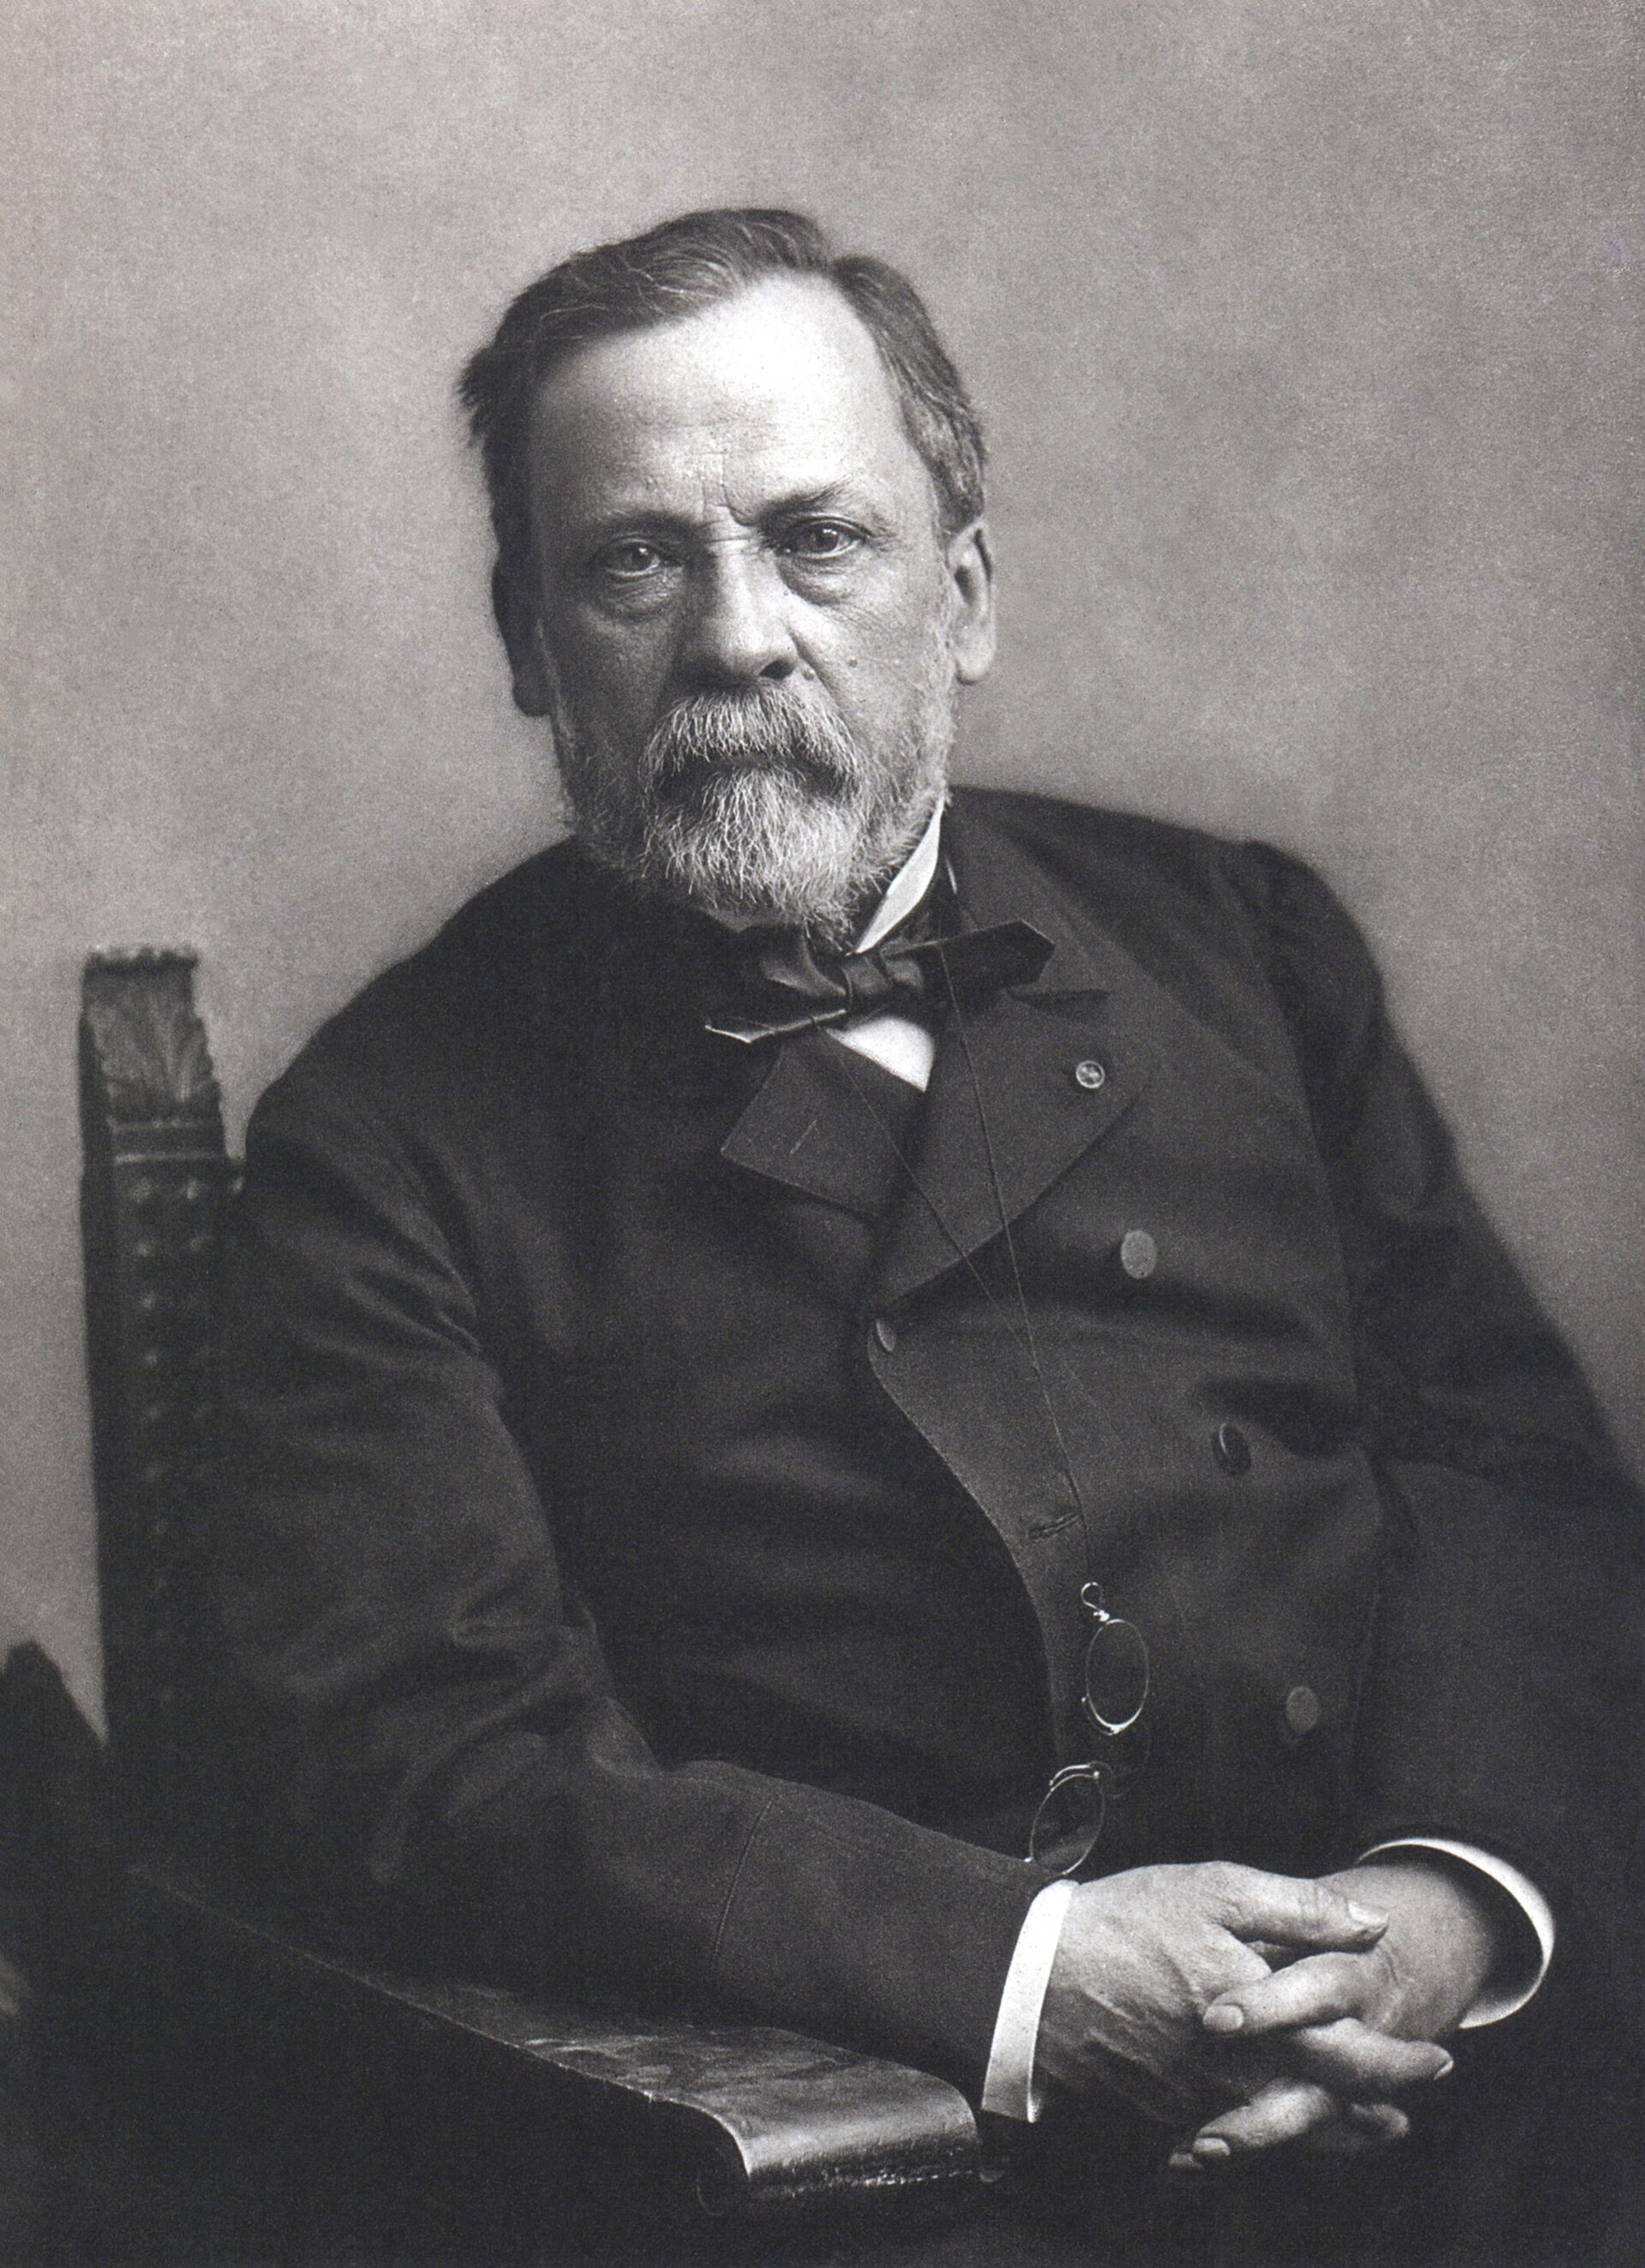
\includegraphics[height=5cm]{images/book1/pasteur.jpg}

{\small Louis Pasteur (1822--1895), fotografado por Paul Nadar.}
\end{minipage}\qquad
\begin{minipage}[t]{0.36\linewidth}\centering
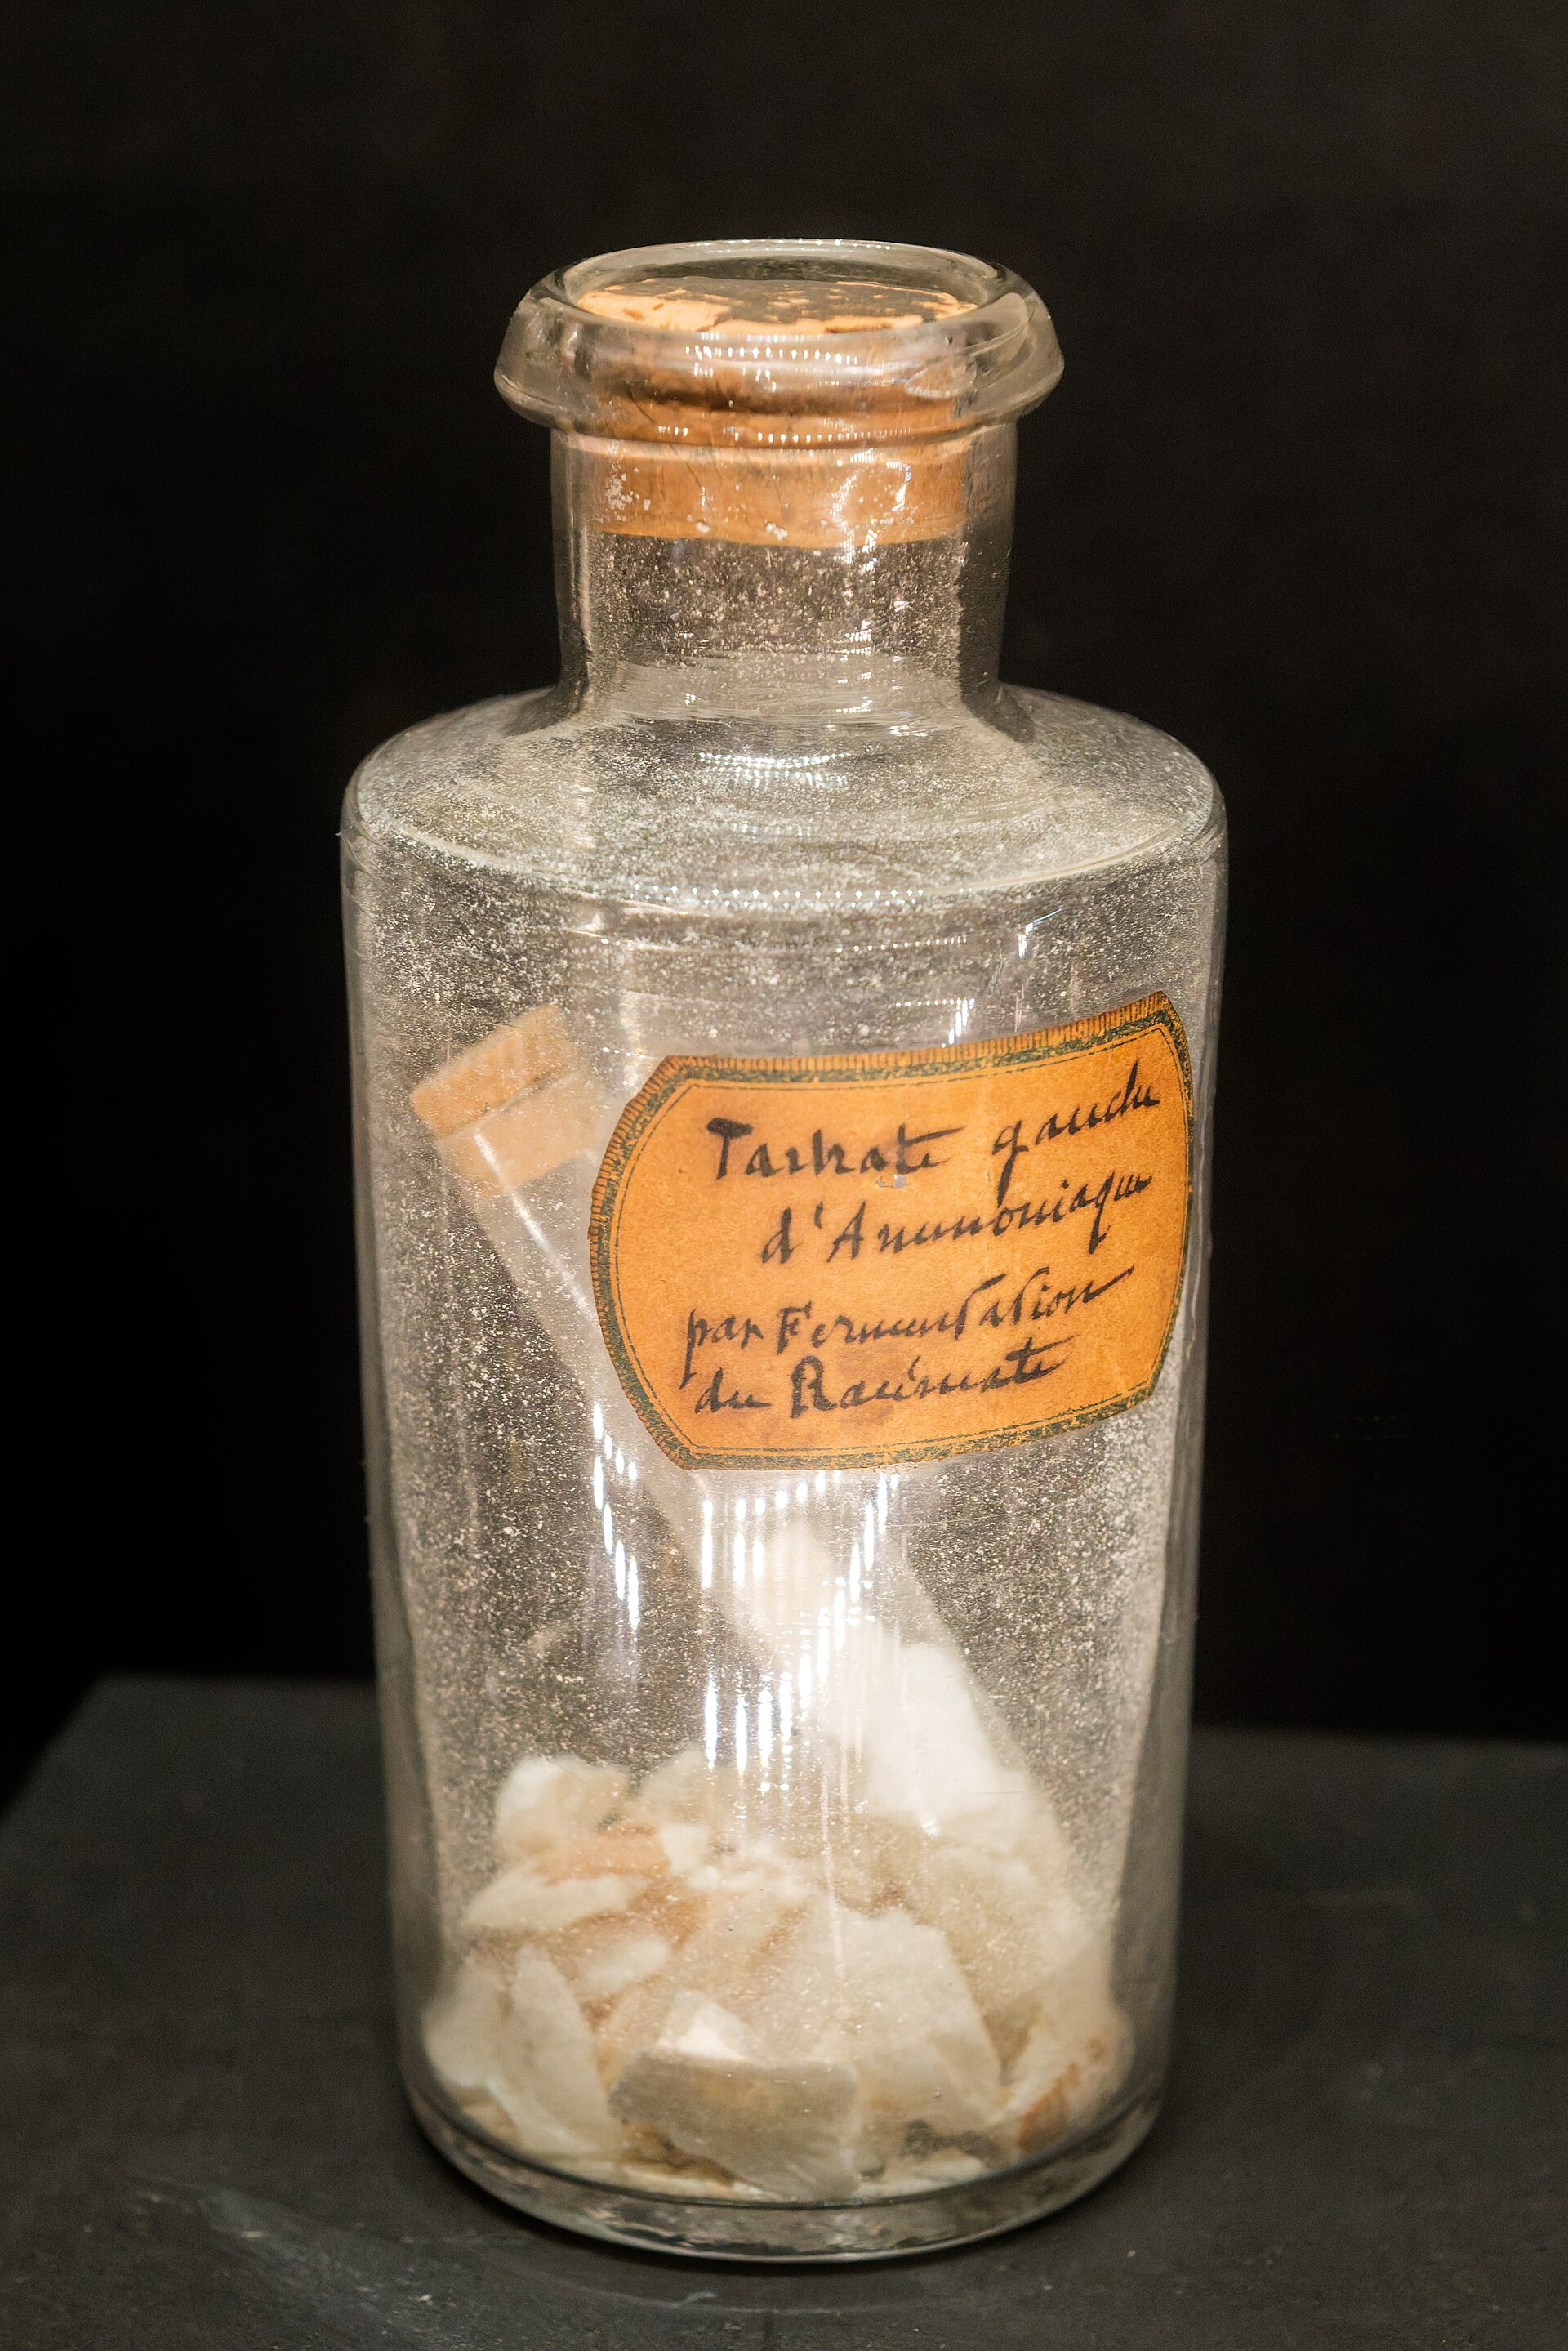
\includegraphics[height=5cm]{images/book1/tartrate-crystals.jpg}

{\small Cristais de tartarato de amônio da coleção de Pasteur. Foto de
Marie-Lan Taÿ Pamart, CC BY 4.0.}
\end{minipage}
\end{omfigure}

\section{Os isômeros Z e E}


\begin{definition}[Isômeros Z e E]\label{def:g12:stereochemistry:z-e}
Quando cada carbono de uma \omterm{def:g10:lewis-and-shape:multiple-bond}{ligação dupla} \ce{C=C} carrega dois \omterm{def:g7:atoms-and-molecules:atom}{átomos} ou
grupos diferentes, existem dois \omterm{def:g12:stereochemistry:stereoisomer}{estereoisômeros}, porque a \omterm{def:g10:lewis-and-shape:multiple-bond}{ligação dupla}
não gira. Em cada carbono, o grupo cujo \omterm{def:g7:atoms-and-molecules:atom}{átomo} ligado a ele tem o maior
\omterm{def:g9:inside-the-atom:atomic-number}{número atômico} tem prioridade. Se os dois grupos prioritários estão do
mesmo lado da \omterm{def:g10:lewis-and-shape:multiple-bond}{ligação dupla}, o \omterm{def:g11:organic-skeletons:isomer}{isômero} é \emph{Z}\index{isomero Z@isômero Z}; se
estão em lados opostos, ele é \emph{E}\index{isomero E@isômero E}.
\end{definition}

\begin{method}[Z ou E?]\label{met:g12:stereochemistry:z-e}
\begin{enumerate}
  \item Verifique que cada carbono da \omterm{def:g10:lewis-and-shape:multiple-bond}{ligação dupla} carrega dois grupos
        diferentes; senão, não há isomeria \omterm{def:g12:stereochemistry:z-e}{Z}/\omterm{def:g12:stereochemistry:z-e}{E}.
  \item Em cada carbono, dê prioridade ao grupo cujo primeiro \omterm{def:g7:atoms-and-molecules:atom}{átomo} tem
        o maior \omterm{def:g9:inside-the-atom:atomic-number}{número atômico} (as regras completas para os empates são
        dadas no volume do primeiro ano da universidade).
  \item Mesmo lado: \omterm{def:g12:stereochemistry:z-e}{Z}. Lados opostos: \omterm{def:g12:stereochemistry:z-e}{E}.
\end{enumerate}
\end{method}

\begin{omfigure}
\setchemfig{atom sep=2em}
\begin{tabular}{cc}
\chemfig{C(-[:150]H_3C)(-[:210]H)=C(-[:30]CH_3)(-[:-30]H)} &
\chemfig{C(-[:150]H_3C)(-[:210]H)=C(-[:30]H)(-[:-30]CH_3)} \\[4pt]
\small (\omterm{def:g12:stereochemistry:z-e}{Z})-but-2-eno: grupos \ce{CH3} do mesmo lado &
\small (\omterm{def:g12:stereochemistry:z-e}{E})-but-2-eno: grupos \ce{CH3} em lados opostos
\end{tabular}

{\small Os dois \omterm{def:g12:stereochemistry:stereoisomer}{estereoisômeros} do but-2-eno. Em cada carbono, o \ce{CH3}
(carbono, $Z = 6$) tem prioridade sobre o \ce{H} ($Z = 1$). Eles são
\omterm{def:g12:stereochemistry:diastereomer}{diastereoisômeros}: fervem a temperaturas diferentes.}
\end{omfigure}

\section{As conformações}

\begin{definition}[Conformação]\label{def:g12:stereochemistry:conformation}
Os \omterm{def:g7:atoms-and-molecules:atom}{átomos} de uma \omterm{def:g7:atoms-and-molecules:molecule}{molécula} podem girar em torno de uma ligação simples.
Cada disposição alcançada por essas rotações é uma
\emph{conformação}\index{conformacao@conformação} da \omterm{def:g7:atoms-and-molecules:molecule}{molécula}. As conformações de uma
\omterm{def:g7:atoms-and-molecules:molecule}{molécula} não são \omterm{def:g11:organic-skeletons:isomer}{isômeros}: elas se transformam umas nas outras o tempo
todo à temperatura ambiente.
\end{definition}

\begin{omfigure}
\begin{tikzpicture}[font=\small]
  \pic (s) at (0,0) {omnewman={90}{30}};
  \foreach \k in {1,2,3} { \node at (s-f\k) {H}; \node at (s-b\k) {H}; }
  \node[anchor=north, align=center] at (0,-1.7) {alternada: os átomos H\\ se alternam};
  \pic (e) at (5,0) {omnewman={90}{112}};
  \foreach \k in {1,2,3} { \node at (e-f\k) {H}; \node[black!60] at (e-b\k) {H}; }
  \node[anchor=north, align=center] at (5,-1.7) {eclipsada: frente a frente\\ (desenhados afastados)};
\end{tikzpicture}

{\small Duas \omterm{def:g12:stereochemistry:conformation}{conformações} do etano, \ce{CH3-CH3}, vistas ao longo da
ligação \ce{C-C}: o carbono da frente é o centro, o carbono de trás é o
círculo. A \omterm{def:g12:stereochemistry:conformation}{conformação} alternada, em que os \omterm{def:g7:atoms-and-molecules:atom}{átomos} estão o mais longe
possível uns dos outros, é a mais estável.}
\end{omfigure}

\begin{remark}[Por que isso importa]\label{rem:g12:stereochemistry:matters}
Os seres vivos são feitos de \omterm{def:g7:atoms-and-molecules:molecule}{moléculas} \omterm{def:g12:stereochemistry:chiral}{quirais} (proteínas, açúcares), e
os receptores e as enzimas feitos delas distinguem os \omterm{def:g12:stereochemistry:enantiomer}{enantiômeros}: dois
\omterm{def:g12:stereochemistry:enantiomer}{enantiômeros} podem ter cheiros, gostos ou efeitos como medicamento muito
diferentes. É por isso que os químicos que fabricam um medicamento com
um \omterm{def:g12:stereochemistry:chiral}{carbono assimétrico} precisam saber que \omterm{def:g12:stereochemistry:enantiomer}{enantiômero} estão fabricando, e
testar cada um.
\end{remark}

\section{Exercícios}

\begin{exercise}[$\star$]\label{exo:g12:stereochemistry:1}
Quais destas \omterm{def:g7:atoms-and-molecules:molecule}{moléculas} têm um \omterm{def:g12:stereochemistry:chiral}{carbono assimétrico}? Marque-o com um
asterisco. Butan-2-ol \ce{CH3-CH(OH)-CH2-CH3}; propan-2-ol
\ce{CH3-CH(OH)-CH3}; 2-clorobutano; ácido lático \ce{CH3-CH(OH)-COOH}.
\end{exercise}

\begin{exercise}[$\star$]\label{exo:g12:stereochemistry:2}
Cada \omterm{def:g11:organic-skeletons:isomer}{isômero} é \omterm{def:g12:stereochemistry:z-e}{Z} ou \omterm{def:g12:stereochemistry:z-e}{E}?
\begin{center}
\setchemfig{atom sep=1.8em}
\chemfig{C(-[:150]Cl)(-[:210]H)=C(-[:30]Cl)(-[:-30]H)} \qquad
\chemfig{C(-[:150]H_3C)(-[:210]H)=C(-[:30]H)(-[:-30]CH_2-CH_3)}
\end{center}
\end{exercise}

\begin{exercise}[$\star$]\label{exo:g12:stereochemistry:3}
Quais são \omterm{def:g12:stereochemistry:chiral}{quirais}: uma luva, uma colher, um parafuso, um cubo? Qual das
\omterm{def:g7:atoms-and-molecules:molecule}{moléculas} \ce{CH2Cl2} e \ce{CHFClBr} é \omterm{def:g12:stereochemistry:chiral}{quiral}?
\end{exercise}

\begin{exercise}[$\star$]\label{exo:g12:stereochemistry:4}
O que é uma \omterm{def:g12:stereochemistry:enantiomer}{mistura racêmica}? No caso da carvona, ela tem cheiro de
hortelã, de alcaravia ou dos dois?
\end{exercise}

\begin{exercise}[$\star$]\label{exo:g12:stereochemistry:5}
O but-1-eno \ce{CH2=CH-CH2-CH3} pode existir como \omterm{def:g12:stereochemistry:z-e}{isômeros Z} e \omterm{def:g12:stereochemistry:z-e}{E}? Por
quê?
\end{exercise}

\begin{exercise}[$\star\star$]\label{exo:g12:stereochemistry:6}
Desenhe os dois \omterm{def:g12:stereochemistry:enantiomer}{enantiômeros} do butan-2-ol na \omterm{def:g12:stereochemistry:cram}{representação de Cram}, com
um espelho entre eles.
\end{exercise}

\begin{exercise}[$\star\star$]\label{exo:g12:stereochemistry:7}
Quantos \omterm{def:g12:stereochemistry:stereoisomer}{estereoisômeros} têm: o 2-clorobutano; o 2,3-diclorobutano
\ce{CH3-CHCl-CHCl-CH3}; o pent-2-eno \ce{CH3-CH=CH-CH2-CH3}?
\end{exercise}

\begin{exercise}[$\star\star$]\label{exo:g12:stereochemistry:8}
Diga se estes pares são \omterm{def:g12:stereochemistry:enantiomer}{enantiômeros}, \omterm{def:g12:stereochemistry:diastereomer}{diastereoisômeros} ou a mesma
\omterm{def:g7:atoms-and-molecules:molecule}{molécula}: os ácidos L- e D-tartárico; os ácidos L- e meso-tartárico; o
(\omterm{def:g12:stereochemistry:z-e}{Z})- e o (\omterm{def:g12:stereochemistry:z-e}{E})-but-2-eno; o ácido meso-tartárico e a sua própria imagem no
espelho.
\end{exercise}

\begin{exercise}[$\star\star$]\label{exo:g12:stereochemistry:9}
O butano, \ce{CH3-CH2-CH2-CH3}, visto ao longo da sua ligação central.
Desenhe a \omterm{def:g12:stereochemistry:conformation}{conformação} alternada em que os dois grupos \ce{CH3} estão
opostos, e uma eclipsada em que eles ficam frente a frente. Qual é a
mais estável? Por quê?
\end{exercise}

\begin{exercise}[$\star\star$]\label{exo:g12:stereochemistry:10}
O ácido meso-tartárico tem dois \omterm{def:g12:stereochemistry:chiral}{carbonos assimétricos}, mas não é \omterm{def:g12:stereochemistry:chiral}{quiral}.
Explique, usando o seu plano de simetria.
\end{exercise}

\begin{exercise}[$\star\star$]\label{exo:g12:stereochemistry:11}
Desenhe e dê nome aos \omterm{def:g12:stereochemistry:z-e}{isômeros Z} e \omterm{def:g12:stereochemistry:z-e}{E} do pent-2-eno.
\end{exercise}

\begin{exercise}[$\star\star\star$]\label{exo:g12:stereochemistry:12}
O 2,3-dibromobutano \ce{CH3-CHBr-CHBr-CH3} tem dois \omterm{def:g12:stereochemistry:chiral}{carbonos
assimétricos}. Desenhe os seus \omterm{def:g12:stereochemistry:stereoisomer}{estereoisômeros} na representação em
zigue-zague usada para o ácido tartárico, e mostre que um deles é uma
forma meso.
\end{exercise}

\begin{exercise}[$\star\star\star$]\label{exo:g12:stereochemistry:13}
Uma \omterm{def:g7:atoms-and-molecules:molecule}{molécula} de medicamento tem um \omterm{def:g12:stereochemistry:chiral}{carbono assimétrico}. A sua \omterm{def:g10:synthesis-yield:synthesis}{síntese} dá
uma \omterm{def:g12:stereochemistry:enantiomer}{mistura racêmica}, mas só um \omterm{def:g12:stereochemistry:enantiomer}{enantiômero} se encaixa no receptor
\omterm{def:g12:stereochemistry:chiral}{quiral} sobre o qual ele deve agir. Que fração do medicamento racêmico é
ativa? Dê duas maneiras de um químico fazer melhor.
\end{exercise}

\begin{exercise}[$\star\star\star$]\label{exo:g12:stereochemistry:14}
O hexa-2,4-dieno, \ce{CH3-CH=CH-CH=CH-CH3}, tem duas \omterm{def:g10:lewis-and-shape:multiple-bond}{ligações duplas},
cada uma podendo ser \omterm{def:g12:stereochemistry:z-e}{Z} ou \omterm{def:g12:stereochemistry:z-e}{E}. Quantos \omterm{def:g12:stereochemistry:stereoisomer}{estereoisômeros} ele tem? (Cuidado
com a simetria da \omterm{def:g7:atoms-and-molecules:molecule}{molécula}.)
\end{exercise}

\begin{exercise}[$\star\star\star$]\label{exo:g12:stereochemistry:15}
Uma \omterm{def:g7:atoms-and-molecules:molecule}{molécula} de açúcar tem três \omterm{def:g12:stereochemistry:chiral}{carbonos assimétricos} e nenhuma
simetria. Quantos \omterm{def:g12:stereochemistry:stereoisomer}{estereoisômeros} ela pode ter no máximo? Quantos pares
de \omterm{def:g12:stereochemistry:enantiomer}{enantiômeros} isso dá? Quantos \omterm{def:g12:stereochemistry:diastereomer}{diastereoisômeros} tem cada
\omterm{def:g12:stereochemistry:stereoisomer}{estereoisômero}?
\end{exercise}

\section{Problema: os cristais de Pasteur}


\begin{problem}[{Problema de fim de semana --- o ácido tartárico tem dois
carbonos assimétricos: quantos estereoisômeros ele tem de verdade?}]
\label{pb:g12:stereochemistry:1}
% ledger: mp:tartaric-L, aw:C, aw:H, aw:O
As formas do ácido tartárico, \ce{HOOC-CH(OH)-CH(OH)-COOH}, tiveram um
papel decisivo na descoberta de que as \omterm{def:g7:atoms-and-molecules:molecule}{moléculas} podem ter ``mão''. O
ácido L-tartárico funde a cerca de \qty{169}{\celsius}.

\medskip
\noindent\textbf{Parte I --- A \omterm{def:g7:atoms-and-molecules:molecule}{molécula}.}
\begin{enumerate}
  \item Dê a \omterm{def:g11:organic-skeletons:formulas}{fórmula molecular} do ácido tartárico e a sua \omterm{def:g10:the-mole:molar-mass}{massa molar}.
  \item Dê o nome dos seus \omterm{def:g11:functional-groups:functional-group}{grupos funcionais}, e diga quantos há de cada.
  \item Que \omterm{def:g7:atoms-and-molecules:atom}{átomos} de carbono são assimétricos? Liste os quatro grupos de
        cada um.
  \item Segundo a regra deste capítulo, quantos \omterm{def:g12:stereochemistry:stereoisomer}{estereoisômeros} ele
        poderia ter no máximo?
\end{enumerate}

\medskip
\noindent\textbf{Parte II --- Os \omterm{def:g12:stereochemistry:stereoisomer}{estereoisômeros}.}
\begin{enumerate}[resume]
  \item No desenho em zigue-zague do ácido L-tartárico, os grupos
        \ce{OH} são desenhados com cunhas cheias ou tracejadas?
  \item Desenhe a sua imagem no espelho. As duas podem ser sobrepostas?
        Dê o nome da imagem no espelho.
  \item Desenhe a forma com uma cunha cheia e uma tracejada. Gire-a
        mentalmente em torno da ligação central, e encontre um plano de
        simetria.
  \item Essa forma é \omterm{def:g12:stereochemistry:chiral}{quiral}? Como ela se chama?
  \item Explique por que o ácido tartárico só tem três \omterm{def:g12:stereochemistry:stereoisomer}{estereoisômeros}.
  \item Diga se L e D, e depois L e meso, são \omterm{def:g12:stereochemistry:enantiomer}{enantiômeros} ou
        \omterm{def:g12:stereochemistry:diastereomer}{diastereoisômeros}.
\end{enumerate}

\medskip
\noindent\textbf{Parte III --- As propriedades.}
\begin{enumerate}[resume]
  \item A que temperatura funde o ácido D-tartárico? Por quê?
  \item O ácido meso-tartárico tem de fundir na mesma temperatura? Por
        quê?
  \item A carvona mostra que dois \omterm{def:g12:stereochemistry:enantiomer}{enantiômeros} podem ter cheiros
        diferentes. Por que um nariz consegue distingui-los e um
        termômetro não?
  \item Uma \omterm{def:g12:stereochemistry:enantiomer}{mistura racêmica} dos ácidos L- e D-tartárico: é uma
        \omterm{def:g6:pure-substances-and-mixtures:pure-substance}{substância pura}? Ela tem atividade óptica como um todo?
\end{enumerate}

\medskip
\noindent\textbf{Parte IV --- Pasteur.}
\begin{enumerate}[resume]
  \item O sal racêmico de Pasteur deu cristais de duas formas, imagens no
        espelho uma da outra. O que cada cristal continha?
  \item A partir de \qty{10.0}{g} de sal racêmico, que massa de cada tipo
        de cristal ele podia esperar?
  \item Por que a forma meso nunca aparece entre esses cristais?
  \item Como ele podia verificar, depois da separação, que os dois montes
        eram \omterm{def:g12:stereochemistry:enantiomer}{enantiômeros}?
  \item O 3-clorobutan-2-ol, \ce{CH3-CHCl-CH(OH)-CH3}, também tem dois
        \omterm{def:g12:stereochemistry:chiral}{carbonos assimétricos}. Quantos \omterm{def:g12:stereochemistry:stereoisomer}{estereoisômeros} ele tem? Por que
        ele não perde um, como o ácido tartárico?
  \item Dê a resposta final: quantos \omterm{def:g12:stereochemistry:stereoisomer}{estereoisômeros} tem o ácido
        tartárico?
\end{enumerate}
\end{problem}
